\documentclass[7.5pt]{article}

\usepackage{amssymb,amsmath,amsthm,chngcntr,makeidx,fancyhdr,rotating,graphicx,hyperref,mathtools}

\usepackage[a4paper,bottom=3cm,hmargin={2cm,2cm}]{geometry}
%\usepackage[dutch]{babel}
\usepackage[all]{xy}
\usepackage[T1]{fontenc}
%\usepackage{pstricks-add}
\usepackage{booktabs}
\usepackage[demo]{graphicx}
\usepackage{subcaption}
\usepackage[shortlabels]{enumitem}
\usepackage{multicol}
\usepackage[]{tikz}
\usetikzlibrary{intersections,positioning,calc,arrows}
\usepackage{pgf,pgfplots}
\pgfplotsset{compat=1.15}
\usepackage{mathrsfs}
\usepackage{xparse}
\usetikzlibrary{calc,angles,positioning,intersections,quotes,decorations.markings}
\usepackage{setspace}

\usepackage{appendix}

\mathtoolsset{centercolon}

\makeatletter
%\newcommand{\xleftrightarrow}[2][]{\ext@arrow 3359\leftrightarrowfill@{#1}{#2}}
\newcommand{\xdashrightarrow}[2][]{\ext@arrow 0359\rightarrowfill@@{#1}{#2}}
\newcommand{\xdashleftarrow}[2][]{\ext@arrow 3095\leftarrowfill@@{#1}{#2}}
\newcommand{\xdashleftrightarrow}[2][]{\ext@arrow 3359\leftrightarrowfill@@{#1}{#2}}
\def\rightarrowfill@@{\arrowfill@@\relax\relbar\rightarrow}
\def\leftarrowfill@@{\arrowfill@@\leftarrow\relbar\relax}
\def\leftrightarrowfill@@{\arrowfill@@\leftarrow\relbar\rightarrow}
\def\arrowfill@@#1#2#3#4{%
  $\m@th\thickmuskip0mu\medmuskip\thickmuskip\thinmuskip\thickmuskip
   \relax#4#1
   \xleaders\hbox{$#4#2$}\hfill
   #3$%
}
\makeatother

\theoremstyle{plain}
\newtheorem{theorem}[subsection]{Theorem}
\newtheorem{corollary}[subsection]{Corollary}
\newtheorem{proposition}[subsection]{Proposition}
\newtheorem{lemma}[subsection]{Lemma}
\theoremstyle{definition}
\newtheorem{definition}[subsection]{Definition}
\newtheorem{example}[subsection]{Example}

\usepackage{gensymb}

\renewcommand{\baselinestretch}{1.2}
\setcounter{MaxMatrixCols}{20}

\let\epsilon=\varepsilon
\let\phi=\varphi
\let\simeq=\cong


\newcommand{\se}[1]{\begin{equation*}
    \begin{split}
        #1
    \end{split}
\end{equation*}}
\newcommand{\sm}[1]{\left(\begin{smallmatrix}
        #1
\end{smallmatrix}\right)}

\newcommand{\Isom}{\mathsf{Isom}\,}
\newcommand{\A}{\mathbb{A}}
\newcommand{\B}{\mathbb{B}}
\newcommand{\C}{\mathbb{C}}
\newcommand{\D}{\mathbb{D}}
\newcommand{\E}{\mathbb{E}}
\newcommand{\F}{\mathbb{F}}
\newcommand{\G}{\mathbb{G}}
\renewcommand{\H}{\mathbb{H}}
\newcommand{\I}{\mathbb{I}}
\newcommand{\J}{\mathbb{J}}
\newcommand{\K}{\mathbb{K}}
\renewcommand{\L}{\mathbb{L}}
\newcommand{\M}{\mathbb{M}}
\newcommand{\N}{\mathbb{N}}
\renewcommand{\O}{\mathbb{O}}
\renewcommand{\P}{\mathbb{P}}
\newcommand{\RP}{\mathbb{RP}}
\newcommand{\PP}{\mathbb{P}}
\newcommand{\EE}{\mathbb{E}}
\newcommand{\Q}{\mathbb{Q}}
\newcommand{\R}{\mathbb{R}}
\newcommand{\T}{\mathbb{T}}
\newcommand{\U}{\mathbb{U}}
\newcommand{\V}{\mathbb{V}}
\newcommand{\W}{\mathbb{W}}
\newcommand{\X}{\mathbb{X}}
\newcommand{\Y}{\mathbb{Y}}
\newcommand{\Z}{\mathbb{Z}}


\newcommand{\ab}{\mathrm{ab}}
\newcommand{\Aff}{\mathrm{Aff}}
\newcommand{\Aut}{\mathrm{Aut}}
\newcommand{\Syl}{\mathrm{Syl}}

\newcommand{\diag}{\mathrm{diag}}
\newcommand{\End}{\mathrm{End}}
\newcommand{\Hom}{\mathrm{Hom}}
\newcommand{\ggd}{\mathrm{ggd}}
\newcommand{\GL}{\mathrm{GL}}
\newcommand{\gr}{\mathrm{gr}}
\newcommand{\id}{\mathrm{id}}
\renewcommand{\Im}{\mathrm{Im}}
\newcommand{\inh}{\mathrm{inh}}
\newcommand{\Image}{\mathrm{Im}}
\newcommand{\Index}{\mathrm{index}}
\newcommand{\Iso}{\mathrm{E}}
\newcommand{\kar}{\mathrm{char}}
\newcommand{\Ker}{\mathrm{Ker}}\let\ker=\Ker
\newcommand{\kgv}{\mathrm{kgv}}
\newcommand{\OO}{\mathrm{O}}
\newcommand{\ord}{\mathrm{ord}}
\newcommand{\orde}{\mathrm{orde}}
\renewcommand{\Re}{\mathrm{Re}}
\newcommand{\SL}{\mathrm{SL}}
\newcommand{\totgr}{\mathrm{totgr}}

\newcommand{\rectangle}{{\sqsubset\!\!\sqsupset}}

\definecolor{light-gray}{gray}{0.5}

\newcommand{\antwoord}[2]{{\color{light-gray}~\newline\boxed{\parbox[t][]{.99\linewidth}{{\tiny \sf ANSWER \thechapter.\arabic{question}}\\ #1}}\vspace{.2cm}}}


\newcommand{\tikzprent}[2]{\begin{center}\begin{tikzpicture}#1\end{tikzpicture}\\{\it #2}\end{center}}

\newcommand{\<}{\langle}
\renewcommand{\>}{\rangle}

\newcommand{\angstrom}{\textup{\AA}}

\usepackage[
backend=biber,
style=nature
]{biblatex}

\addbibresource{library.bib}

\graphicspath{ {./img/} }

\author{
	Broerse, Mart\thanks{\href{mailto:mart.broerse@student.uva.nl}{mart.broerse@student.uva.nl}}\\
	\and
	Jaspers, Boris\thanks{\href{mailto:boris.jaspers@student.uva.nl}{boris.jaspers@student.uva.nl}}\\
	\and
	Marshall, Max\thanks{\href{mailto:max.marshall@student.uva.nl}{max.marshall@student.uva.nl}}
}

\title{%
  Optimization of the Power Factor for High Temperature Applications by Manipulation of Point Defects \\
  \large Workshop Physics and Astronomy \\ Institute for Theoretical Physics Amsterdam}
  
\date{January 2023}


\begin{document}

\maketitle

% mart's settings, setstretch 1.157, lettertype 7.5
\setstretch{1.157}

% TODO walk through checklist in slides
% [more detailed background 2]
% [general problem 1]
% [main result]
% [how problem adds to knowledge]
\begin{abstract}
\noindent Thermoelectrics are materials that can be used to directly convert heat into electrical energy \cite{CHAMPIER2017167}.
Recently, molybdenum silicides have garnered the interest of scientists within the field of thermoelectrics for their high melting points and favourable corrosion resistance \cite{Lian2009}. 
However, the available information regarding the different molybdenum sillicides is lacking at present.
Here, we show the predicted power factor and other transport properties of trimolybdenum disillicide ($\text{Mo}_3\text{Si}_2$) evaluated with Density Functional Theory (DFT) for four intrinsic point defects at high temperatures; contrasted with the transport properties of molybdenum disillicide ($\text{Mo}\text{Si}_2$).
% The stability of each point defect was determined by calculating the equilibrium defect concentration.
We conclude that $\text{Mo}_3\text{Si}_2$ does not appear to be a promising thermoelectric material, with a maximum power factor of 1.5 $m$W/m\cdot $\text{K}^2$ at 1800 K, significantly less than that of hexagonal $\text{MoSi}_2$ at 7.7 $m$W/m\cdot $\text{K}^2$. 
All point defects studied were predicted to have a negative impact on the power factor of $\text{Mo}_3\text{Si}_2$. 
Despite these results $\text{Mo}_3\text{Si}_2$ as a thermoelectric still warrants further investigation, as our method can be improved upon.
Two potential experimental methods are presented to aid similar studies in verifying such results: one for characterizing the point defects in the volume of the material, and one for obtaining high-resolution data on density of states. 

\end{abstract}

\section{Introduction}
\begin{multicols}{2}
\noindent Thermoelectrics have the potential to play a key role in addressing one of this generation's defining crises, namely the increasing demand for sustainable energy \cite{Wang2021}. These materials can be utilised to directly convert waste heat into electrical energy, which could significantly improve the energy efficiency of processes that generate excess heat \cite{Wang2021}.
The applications of thermoelectric materials are not limited to bulk waste heat recovery; they can also be applied in devices that require precise or localised temperature control \cite{1616249}.
Thermoelectrics are solid state materials, and as a result need less maintenance and space than mechanical electric generators; they do not produce noise, and experience no mechanical wear \cite{SnyderGJeffrey2008Ctm}.

Examples of current Thermoelectric Energy Generation (TEG) applications include: appliances designed for areas with a shortage of electricity, waste heat recovery from vehicles and cargo vessels, power supplies for wireless sensors and wearable devices, and the radioisotope TEG adopted in spacecrafts by the National Aeronautics and Space Administration (NASA) \cite{CHAMPIER2017167, doi:10.2514/6.2005-5713, 10.4108/icst.bodynets.2014.257119}.  
The relatively niche market for TEG is mainly ascribed to the low TE energy conversion efficiency, high cost of TE materials, and slow progress of reliable module development \cite{doi:10.1179/095066003225010182}.

One of the main drawbacks of thermoelectric materials is their low energy conversion efficiency; this makes them less desirable as a solution to the increasing demand for clean energy \cite{SnyderGJeffrey2008Ctm}.
Other problems for the large-scale application of thermoelectrics include the toxicity of the materials and the scarcity of the elements the materials are synthesised from, which consequently affects their cost \cite{LiuWei2017Ehst}.

Some known well-performing thermoelectric materials include V\textsubscript{2}VI\textsubscript{3} compounds and their derivatives, where $\text{V} \in \{\text{Sb}, \text{Bi}\}$ and $\text{VI} \in \{\text{S}, \text{Se}, \text{Te}\}$; these compounds have been used for 60 years and have at multiple times been considered mature \cite{https://doi.org/10.1002/advs.201600004}. 
More recently, $\text{MoSi}_{2}\text{N}_{4}$ has been used to construct a monolayer with potential for applications in catalysis and nanoelectronics \cite{MA2022153214}.

Molybdenum silicides may be suitable candidates for TE materials as they are relatively non-toxic to humans, and while molybdenum is not an abundant element, molybdenum silicides may well be viable for industrial applications \cite{NOVOTNY2018272, HENCKENS201861, STOLOFF20001313}.
Their corrosion resistance and high melting point are desirable properties for such applications; the latter positively affects the range of temperatures at which the material is stable \cite{Nozariasbmarz_2017}.
Molybdenum silicides are stable at a variety of different stoichiometric ratios, but in this paper we only investigate pristine $\text{MoSi}_2$ and $\text{Mo}_3\text{Si}_2$ structures, alongside four defect-containing structures of the latter.
 
The key measure of the quality of a thermoelectric material is its dimensionless figure of merit,

\begin{equation}
z T=\frac{\sigma S^2}{\kappa_{e} + \kappa_{p}}T,
\label{eq:zt}
\end{equation}
 which is a function of temperature T, thermal conductivity $\kappa$ due to electrons and phonons, electrical conductivity $\sigma$ and the Seebeck coefficient $S$.
These parameters can be altered by introducing defects into the material lattice, and are highly correlated in a counteracting way \cite{alma9939162912205131}.
A value larger than one is desirable, but the parameter interdependence proves this difficult to achieve \cite{TakabatakeToshiro2014Petc}.
The computational methods we use do not take a key contributor to the value of $zT$ at high temperatures into account: the phonon contribution to the thermal conductivity \cite{cdi_proquest_reports_1030752835}.
We therefore optimized the power factor $\sigma S^2$ instead, but we note that an increased power factor does not necessarily imply a better $zT$.

It is the subject of this study to investigate the power factor of $\text{Mo}_3\text{Si}_2$ and $\text{MoSi}_2$ at high temperatures. 
Although the power factor can be tuned using several types of defects, the focus of this paper lies on intrinsic point defects, such as vacancies and antisites \cite{alma9939163749005131}. 
Vacancies are vacant sites in the lattice, and an antisite is an atom on a site that should be occupied by another atom in the pristine structure.
The power factor was characterized by means of computational analysis on band energy data, which has been obtained in previous research using Density Functional Theory (DFT).

% REPHRASE - this is copied from a source
% Point defects are atomic scale 0-dimensional (0D) defects including
% vacancies, interstitials, substitutions, Frenkel defects, Schottky
% defects, antisite defects, and what we recently refer to as discordant
% atoms.
% Point defects can be introduced by adjusting the initial reaction stoichiometry or through post synthetic treatment, such as hot deformation, electron irradiation, plasma treatment, and ion implantation.
%--
% The maximum power efficiency of a TE material is defined by
% \begin{equation}
% \eta=\frac{T_{\mathrm{H}}-T_{\mathrm{C}}}{T_{\mathrm{H}}}\left[\frac{\sqrt{1+Z T_{\mathrm{ave}}}-1}{\sqrt{1+Z T_{\mathrm{ave}}}+\frac{T_{\mathrm{C}}}{T_{\mathrm{H}}}}\right],
% \end{equation}
% where T_{H} and T_{C} correspond to the temperatures of the hot and cold sides, respectively. And ZT_{ave} is the device figure of merit value between T_{H} and T_{C}, and the dimensionless figure of merit, ZT, is defined by $ZT=S^{2}\sigma T/\kappa$, where S, σ, and κ are the Seebeck coefficient, electrical conductivity and thermal conductivity of a TE material at a specific temperature T.


\end{multicols}

\pagebreak
\section{Methodology}

\begin{multicols}{2}
\noindent Each of the parameters in the figure of merit depends on the carrier density $C$, temperature $T$ and chemical potential $\mu$; each parameter is also a function of the other, but we took the parameters to be independent of one another by approximation \cite{alma9939162912205131}.
We analyzed the data of the pristine lattice, and of the lattices containing an anti-site or a vacancy; for each of these samples, the transport properties were calculated and varied as a function of the aforementioned parameters: $T$, $\mu$, and the carrier concentration. 
The transport properties were then analyzed to find the structure most favourable as a thermoelectric material.

In order to determine the stability of each of the defects, the equilibrium defect concentration was calculated for the intrinsic defects.
The defect concentration is given by

% TODO C_0!

\begin{equation}
C_{\text {def }}=e^{\frac{-E_f}{k_B T}},
\label{eq:defectconcentration}
\end{equation}

\noindent where $C_{\text {def}}$ is the equilibrium defect concentration, $k_B$ is Boltzmann's constant, $T$ is the temperature, and $E_f$ is the defect formation energy.
The latter is defined as

\begin{equation}
E_f=\left(E_{\text {def}}-\sum n_i \mu_i\right)-E_{\text {pri}},
\label{eq:formationenergy}
\end{equation}

\noindent with $E_\text{def}$ the energy of the defective system, $n$ the number of bonds that are formed, $\mu$ the chemical potential of the atoms, and $E_{\text {pri}}$ the energy of the pristine system.

The simulation data was processed using BoltZTraP2; a python package used to interpolate data obtained by DFT simulations to extract information from the band structure of the materials \cite{MadsenGeorgK.H.2018Bapf}. 
BoltZTraP2 operates under the Constant Relaxation Time Approximation (CRTA); the relaxation time represents the time it takes for an excited system to return to equilibrium. 
A large value corresponds to a short mean free path, which results in more frequent electron and phonon scattering, decreasing the electrical and thermal conductivity respectively \cite{TakabatakeToshiro2014Petc}. 

SeeK-path was used to find high-symmetry points in the lattice, which allowed us to plot the projected band structure through the most relevant points in momentum space (k-space) \cite{HINUMA2017140, togo, HjorthLarsen_2017, qe-tools, ONG2013314}.
It was also used to determine the space group of the various compound structures.
Pymatgen was used to visualise parameter relations to the properties in question \cite{ONG2013314}.
Bond lengths and bond counts were obtained with ASE \cite{ase-paper, ISI:000175131400009}.
Finally, VESTA was used to visualise the three dimensional structure of the lattices and their defects \cite{Momma:ko5060, Momma:db5098}.

\end{multicols}

\smallskip
% \clearpage
\section{Results}

% TODO introduce results

% REPHRASE - this is copied from a source
% Vacancies possess larger mass difference and larger strain fluctuation than the antisite defects, thus more effectively scattering heat-carrying phonons.
% Intrinsic point defects can be created and manipulated compositionally, mechanically (via "the donor-like effect"), and thermally (via "the recovery effect").

\subsection{Material Structure}

\begin{multicols}{2}

\noindent The pristine $\text{Mo}_3\text{Si}_2$ structure is tetragonal and of primitive type, such that $a=b=6.62471$ and $c=3.29545$; $\alpha=\beta=\gamma=90 \degree$.
The four $\text{Mo}_3\text{Si}_2$ defect structures are tetragonal as well, and all are of primitive type, but their spatial dimensions are instead $a=b=13.24581$, $c=13.18552$.
The hexagonal phase of $\text{MoSi}_2$ is of primitive type, with $a=b=4.61480$ and $c=6.61024$; $\alpha=\beta=90 \degree$ and $\gamma=120 \degree$. 
The tetragonal phase is also of primitive type, however the unit-cell was chosen differently; in this paper we use a unit-cell with $a=b=c=4.54748$, $\alpha=\beta=138.5582 \degree$ and $\gamma=138.5582 \degree$ to minimize the cell volume (\autoref{tab:structure}).

The pristine $\text{Mo}_3\text{Si}_2$ compound has roughly as many Mo-Si bonds as the hexagonal phase of the pristine $\text{MoSi}_2$ compound (\autoref{tab:mo-bonds}).
The former has a smaller average bond length than both phases of the pristine $\text{MoSi}_2$ compound, and the minimal bond length rises significantly for the Si vacancy compared to the other $\text{Mo}_3\text{Si}_2$ defects.
The maximal bond length for the $\text{Mo}_\text{Si}$ defect rises significantly as well.
%Mo3Si2-VSi notably has two bonds less than the Mo vacancy compound.

\end{multicols}

% TODO compare with experiment
\begin{table}[t!]
  \small
  \centering
  \caption{The different sample structures, classified by crystal family and space group. Additionally, the unit cell volume is displayed.}
\begin{tabular}{@{}llll@{}}
\toprule
\text {Compound} & \text{Crystal family} & \text{Space group} & \text{Unit-cell volume ($\angstrom^3$)} \\
\midrule
\text{Mo}_3\text{Si}_2\text{ prist.} & \text{Tetragonal} & \text{P4/mbm (number 127)} & 144.6 \\
\text{Mo}_3\text{Si}_2\text{-MoSi} & \text{Tetragonal} & \text{Amm2 (number 38)} & 2313.4 \\
\text{Mo}_3\text{Si}_2\text{-SiMo} & \text{Tetragonal} & \text{Amm2 (number 38)} & 2313.4\\
\text{Mo}_3\text{Si}_2\text{-VMo} & \text{Tetragonal} & \text{Amm2 (number 38)} & 2313.4 \\
\text{Mo}_3\text{Si}_2\text{-VSi} & \text{Tetragonal} & \text{Amm2 (number 38)} & 2313.4 \\
\text{Mo}\text{Si}_2\text{ prist. tetra.} & \text{Tetragonal} & \text{I4/mmm (number 139)} & 40.8  \\
\text{Mo}\text{Si}_2\text{ prist. hexa.} & \text{Hexagonal} & \text{P6-222 (number 180)} & 121.9
\end{tabular}
  \label{tab:structure}
\end{table}

% TODO compare with experiment
\begin{table}[t!]
  \small
  \centering
  \caption{The number of Mo-Si bonds and their minimum, maximum and average bond length (BL).}
\begin{tabular}{@{}lllll@{}}
\toprule
\text {Compound} & \text{Num. bonds} & \text{Min BL (\angstrom)} & \text{Max BL (\angstrom)} & \text{Avg BL (\angstrom)} \\
\midrule
\text{Mo}_3\text{Si}_2\text{ prist.} & 20 & 2.527 & 2.584 & 2.565 \\
\text{Mo}_3\text{Si}_2\text{-MoSi} & 507 & 2.471 & 3.020 & 2.562 \\
\text{Mo}_3\text{Si}_2\text{-SiMo} & 511 & 2.460 & 2.831& 2.564 \\
\text{Mo}_3\text{Si}_2\text{-VMo} & 506 & 2.491 & 2.723 & 2.564 \\
\text{Mo}_3\text{Si}_2\text{-VSi} & 504 & 2.564 & 2.632 & 2.562 \\
\text{Mo}\text{Si}_2\text{ prist. tetr.} & 2 & 2.620 & 2.620 & 2.620 \\
\text{Mo}\text{Si}_2\text{ prist. hexa.} & 18 & 2.581 & 2.654 & 2.605
\end{tabular}
  \label{tab:mo-bonds}
\end{table}

\begin{figure}
\label{fig:mat-pristine}
\centering
\includegraphics[width=0.6\textwidth]{img/Mo3Si2-pristine}
\caption{The $\text{Mo}_3\text{Si}_2$ pristine structure (space group P4/mbm number 127) pictured once with the $c$ axis pointed towards the camera (I), and once in the standard orientation (II).}
\end{figure}

\begin{figure}
\label{fig:mo3si2-defects-b}
\centering
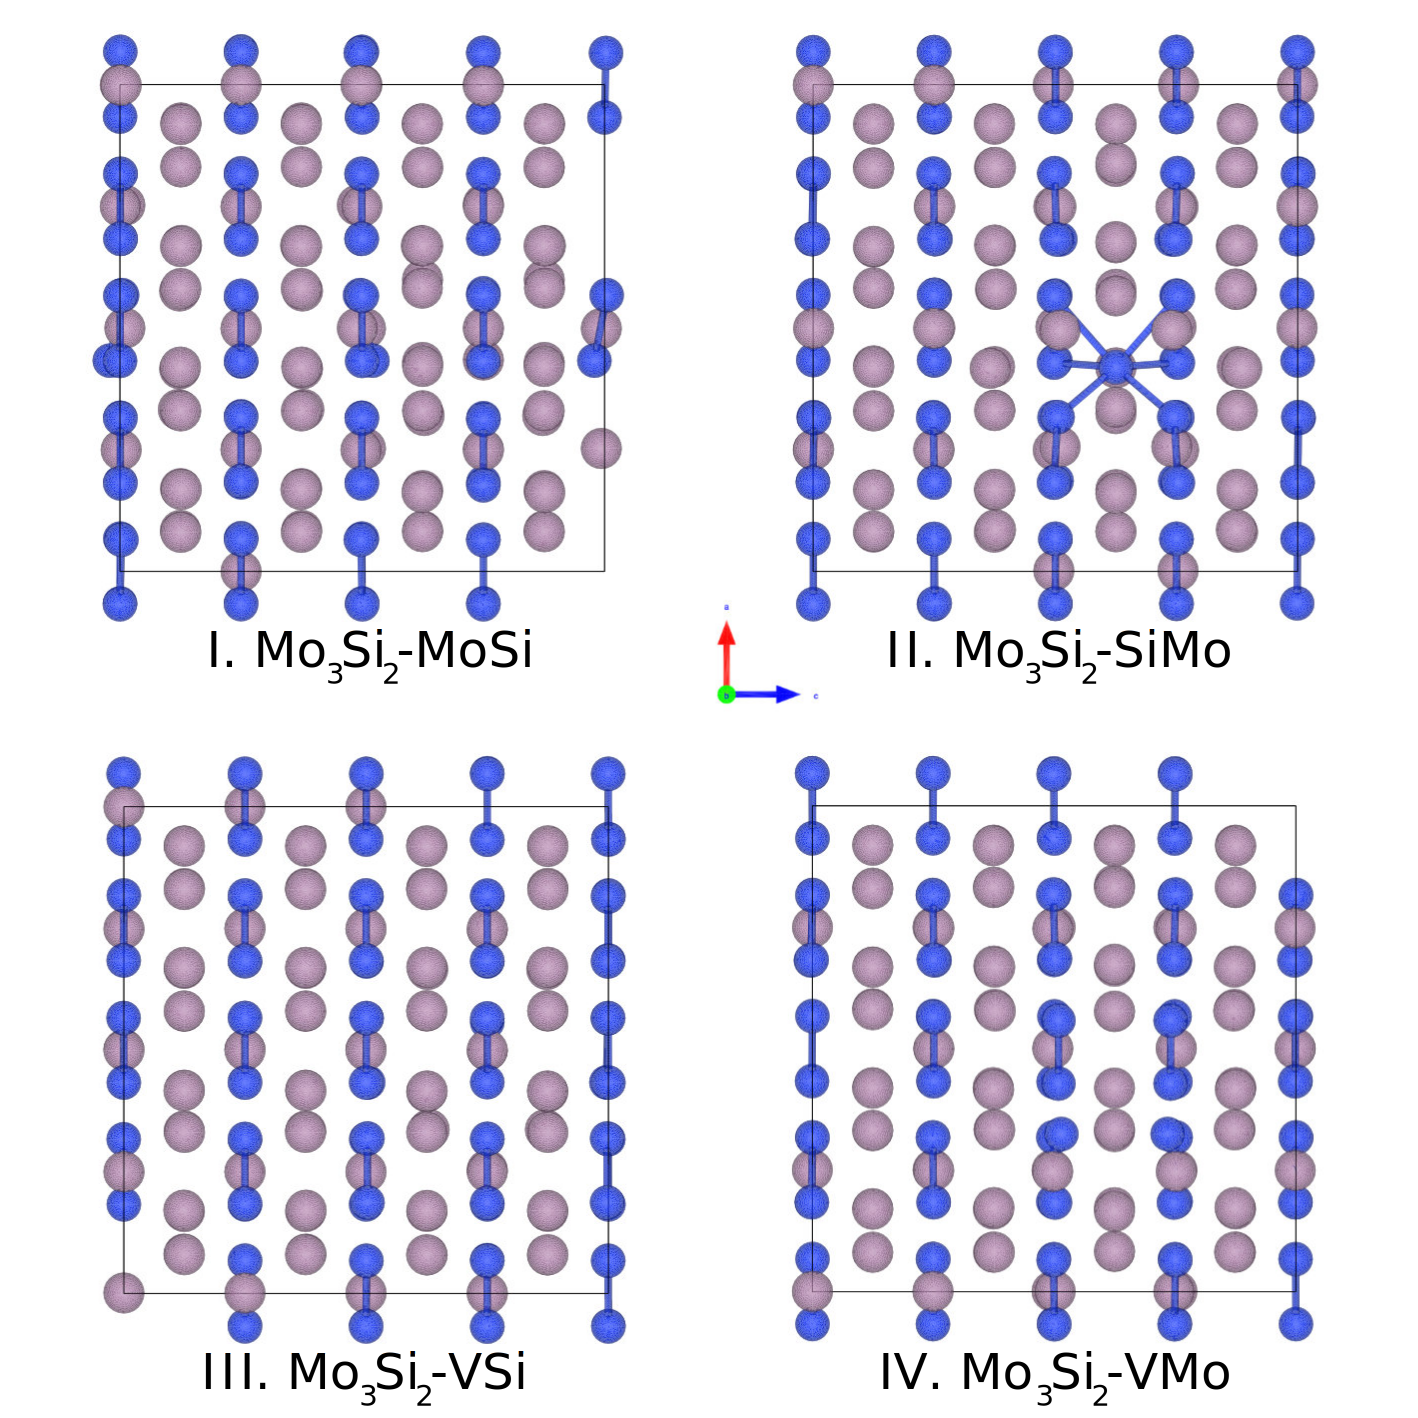
\includegraphics[width=0.5\textwidth]{img/Mo3Si2-defects-b}
\caption{The four defect variants of $\text{Mo}_3\text{Si}_2$ we investigated, all plotted with the $b$ axis facing the camera and the $a$ axis pointing upwards. (I) The $\text{Mo}_{\text{Si}}$ defect (space group Amm2 number 38), which gives rise to a tilted substructure with respect to the pristine lattice, to be seen on the rightmost edge. (II) The $\text{Si}_{\text{Mo}}$ defect (space group Amm2 number 38), with more strongly bonded atoms than the pristine. (III) The silicon vacancy defect (space group Amm2 number 38); and (IV) the molybdenum vacancy defect (space group Amm2 number 38).}
\end{figure}

\begin{figure}
\centering
\begin{subfigure}{0.4\textwidth}
  \centering
  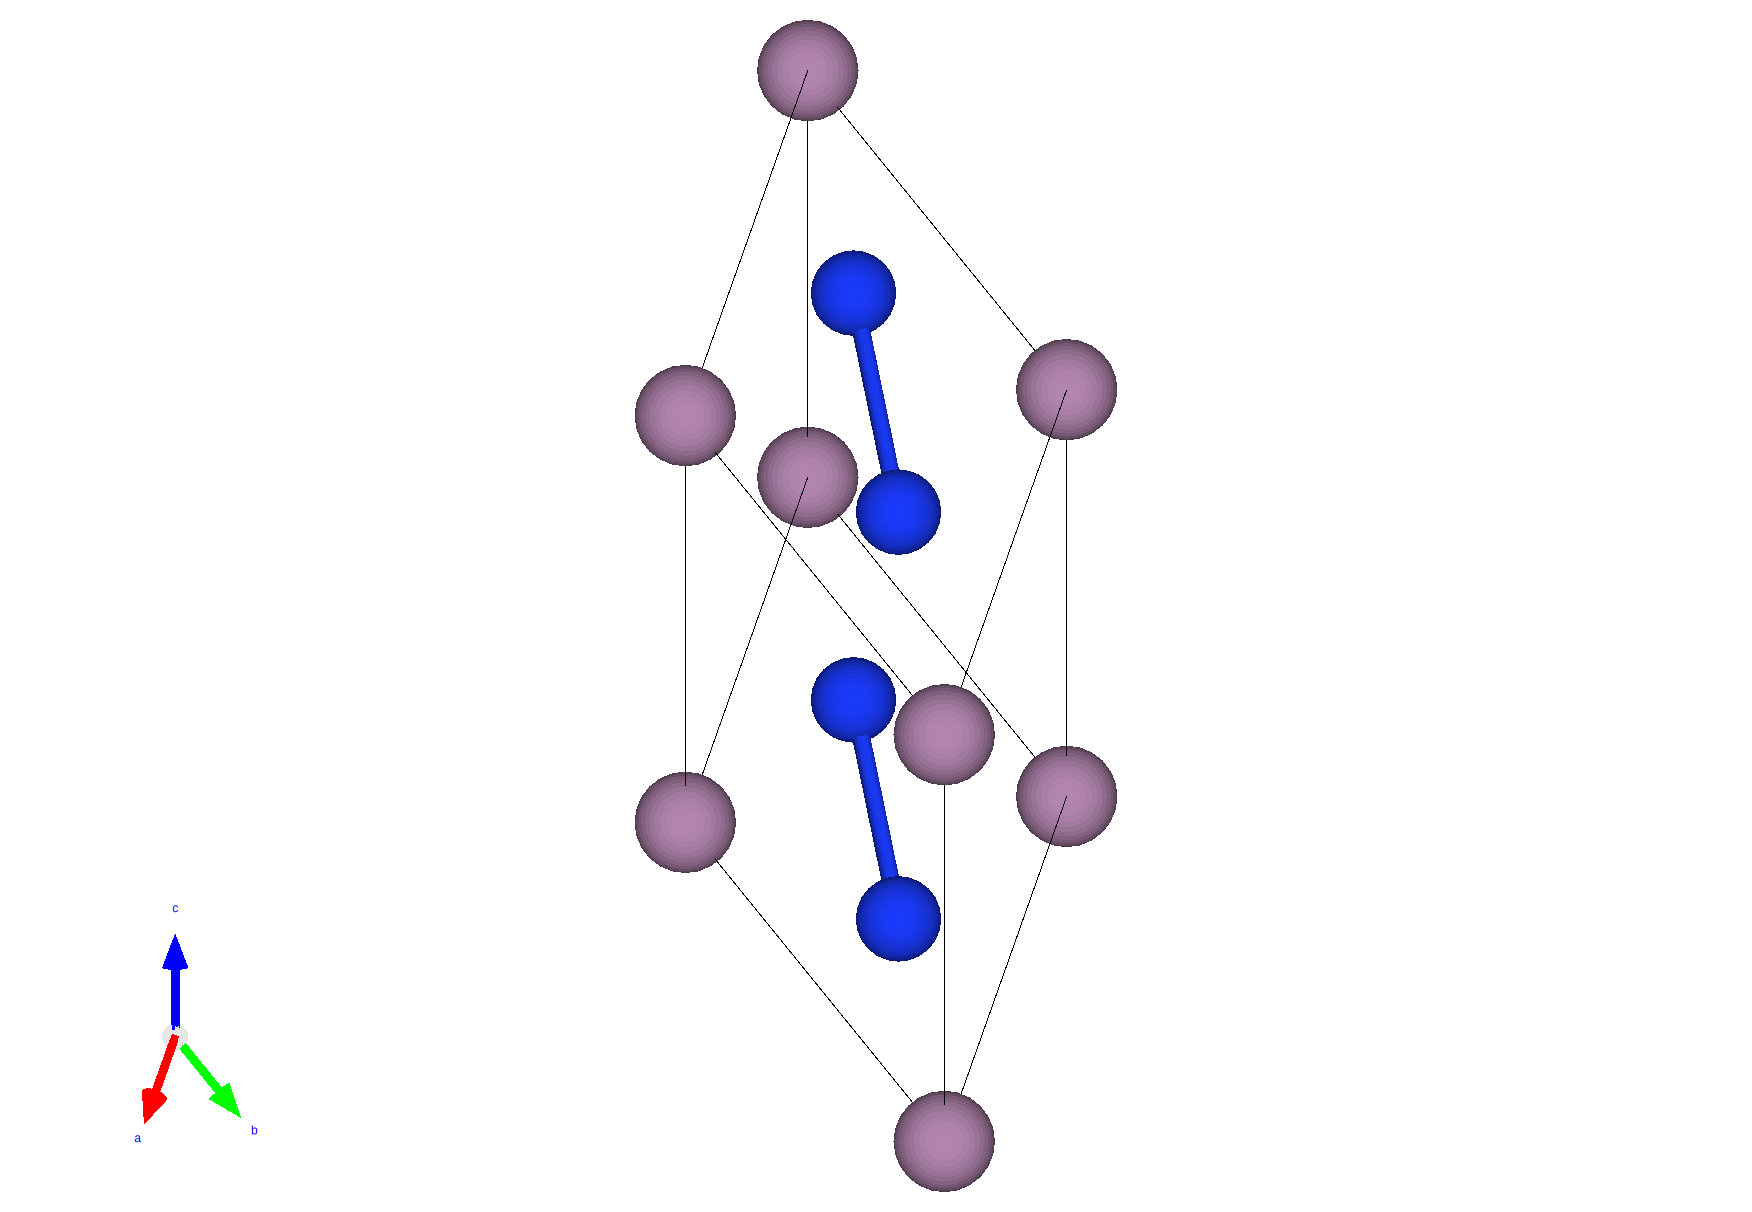
\includegraphics[width=\linewidth]{MoSi2-tetragonal-std}
  \caption{}
\label{fig:mosi2-tetra}
\end{subfigure}%
\begin{subfigure}{.4\textwidth}
  \centering
  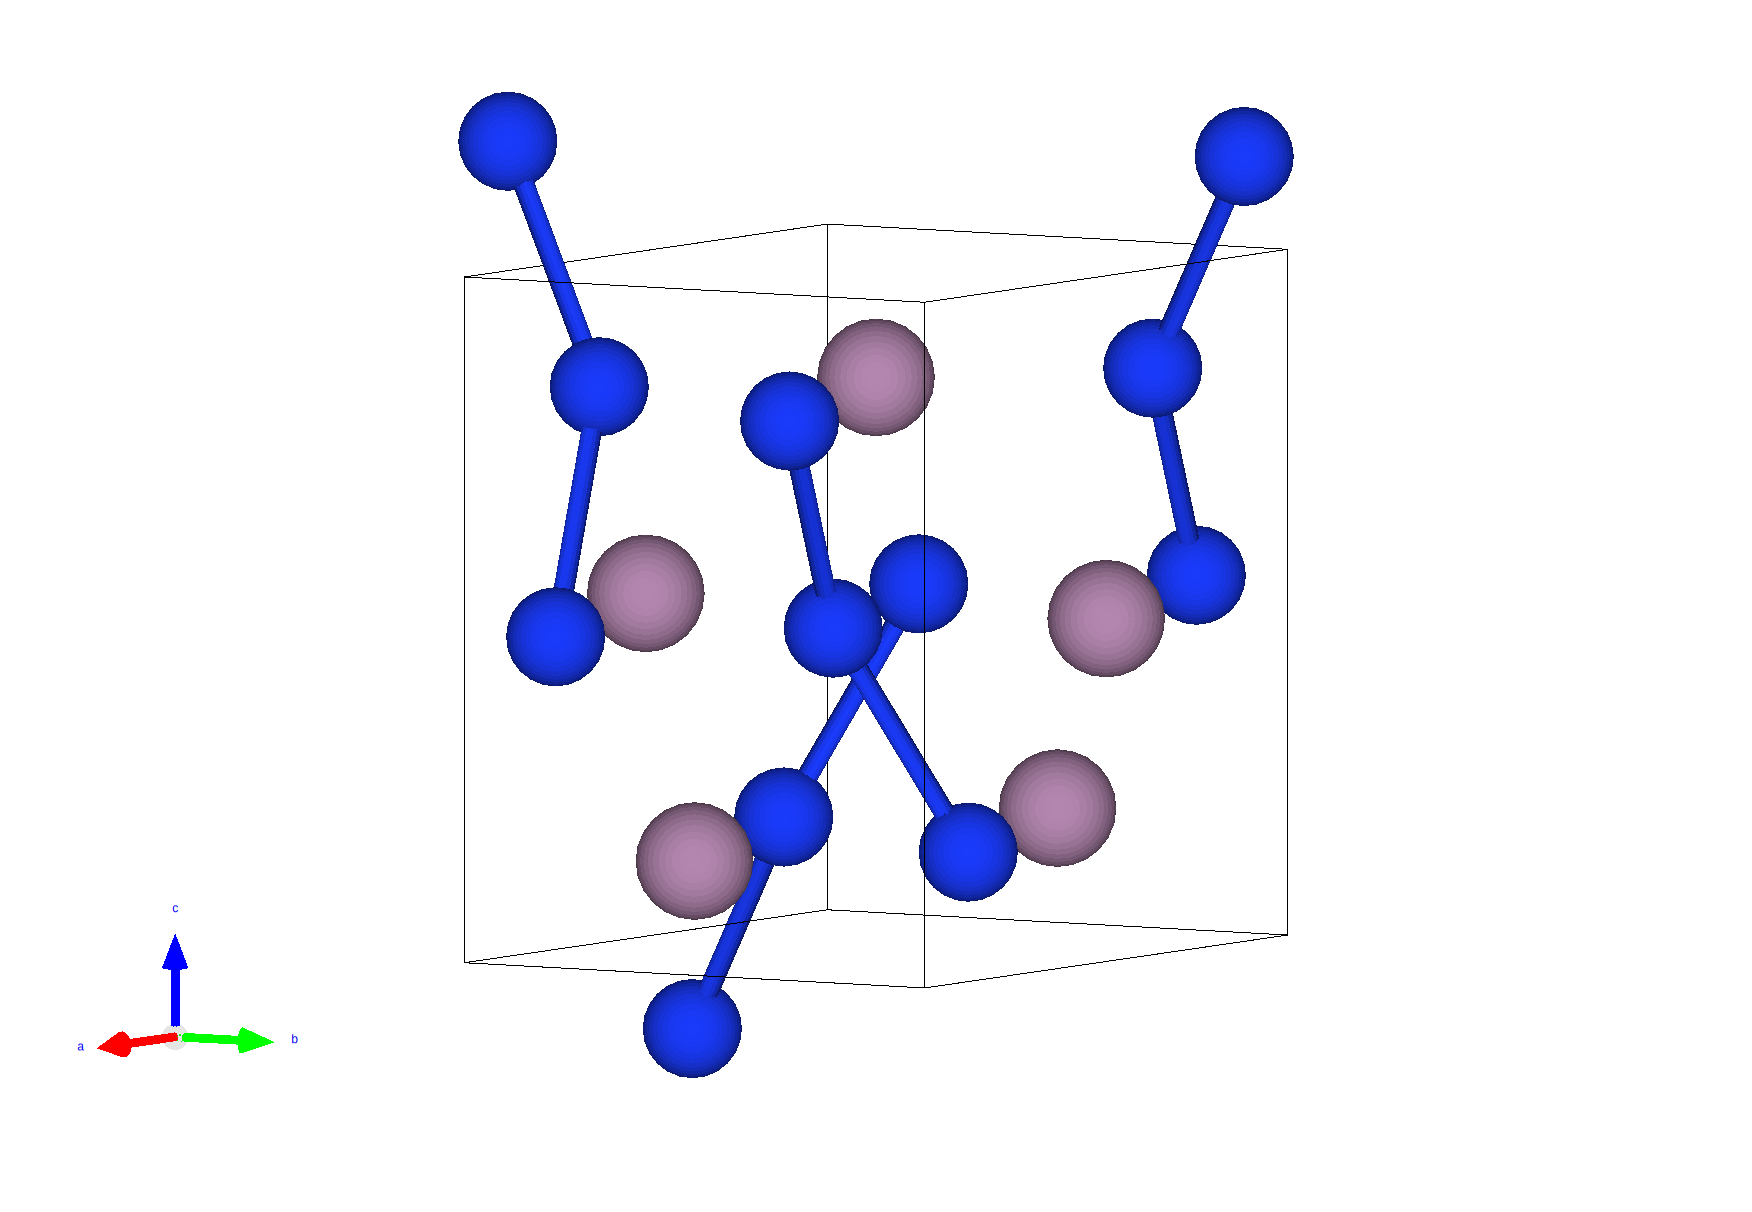
\includegraphics[width=0.75\linewidth]{MoSi2-hexagonal-std}
  \caption{}
\label{fig:mosi2-hexa}
\end{subfigure}
\caption{The pristine tetragonal (a) and hexagonal (b) MoSi\textsubscript{2} structures in the standard orientation.}
\label{fig:MoSi2}
\end{figure}

\clearpage
\subsection{Electronic Band Structure}

\begin{multicols}{2}

 \noindent Whether or not a given compound is a semi-conductor or a metal is determined by its electronic band structure (BS); a material with a BS that has a band gap at the Fermi energy is a semi-conductor, and in absence of such gap a metal.
This classification is essential for correctly identifying material properties from the transport property data. 

Optimizing the electronic band structure involves two key aspects - achieving optimal carrier concentration and increasing the Seebeck coefficient; the former is achieved by adjusting the band filling and the latter through improvement of electronic density of states close to the Fermi level \cite{ZhuTiejun2016NIiI}.
Intrinsic point defects such as vacancies and interstitials are often used to alter the charge carrier concentration or electronic bandwidth \cite{ZhengYun2021Deit}. 

The tetragonal phase of $\text{Mo}\text{Si}_2$ has a low density of states at the Fermi energy, but no band gap; making $\text{Mo}\text{Si}_2$ a semi-metal, whereas the hexagonal phase does have a band gap at the Fermi energy and is therefore a semiconductor (Figures \ref{fig:DOS-mosi2-tetragonal}, \ref{fig:e-plots}). 
$\text{Mo}_3\text{Si}_2$ is predicted to have metal-like properties for similar reasons. 
The presence of the band gap is reflected in the conductivity of electrons near the Fermi energy, as shown in \autoref{fig:e-plots} where bands near the Fermi energy have a lower conductivity for materials with a band gap. 

\end{multicols}


\begin{figure}
\centering
\begin{subfigure}{.32\textwidth}
  \centering
  \includegraphics[width=\linewidth]{bs_MoSi2_tetragonal}
  \caption{}
\label{fig:bs-mosi2-tetra}
\end{subfigure}%
\begin{subfigure}{.32\textwidth}
  \centering
  \includegraphics[width=\linewidth]{bs_MoSi2_hexagonal}
  \caption{}
\label{fig:bs-mosi2-hexa}
\end{subfigure}%
\begin{subfigure}{.32\textwidth}
  \centering
  \includegraphics[width=\linewidth]{bs_Mo3Si2}
  \caption{}
\label{fig:bs-mo3si2}
\end{subfigure}
\caption{The band structure of the tetragonal (a) and hexagonal (b) phases of pristine MoSi\textsubscript{2}, and the pristine Mo\textsubscript{3}Si\textsubscript{2} structure (c) across high symmetry points.}
\label{fig:bs_MoSi2}
\end{figure}

\begin{figure}
\centering
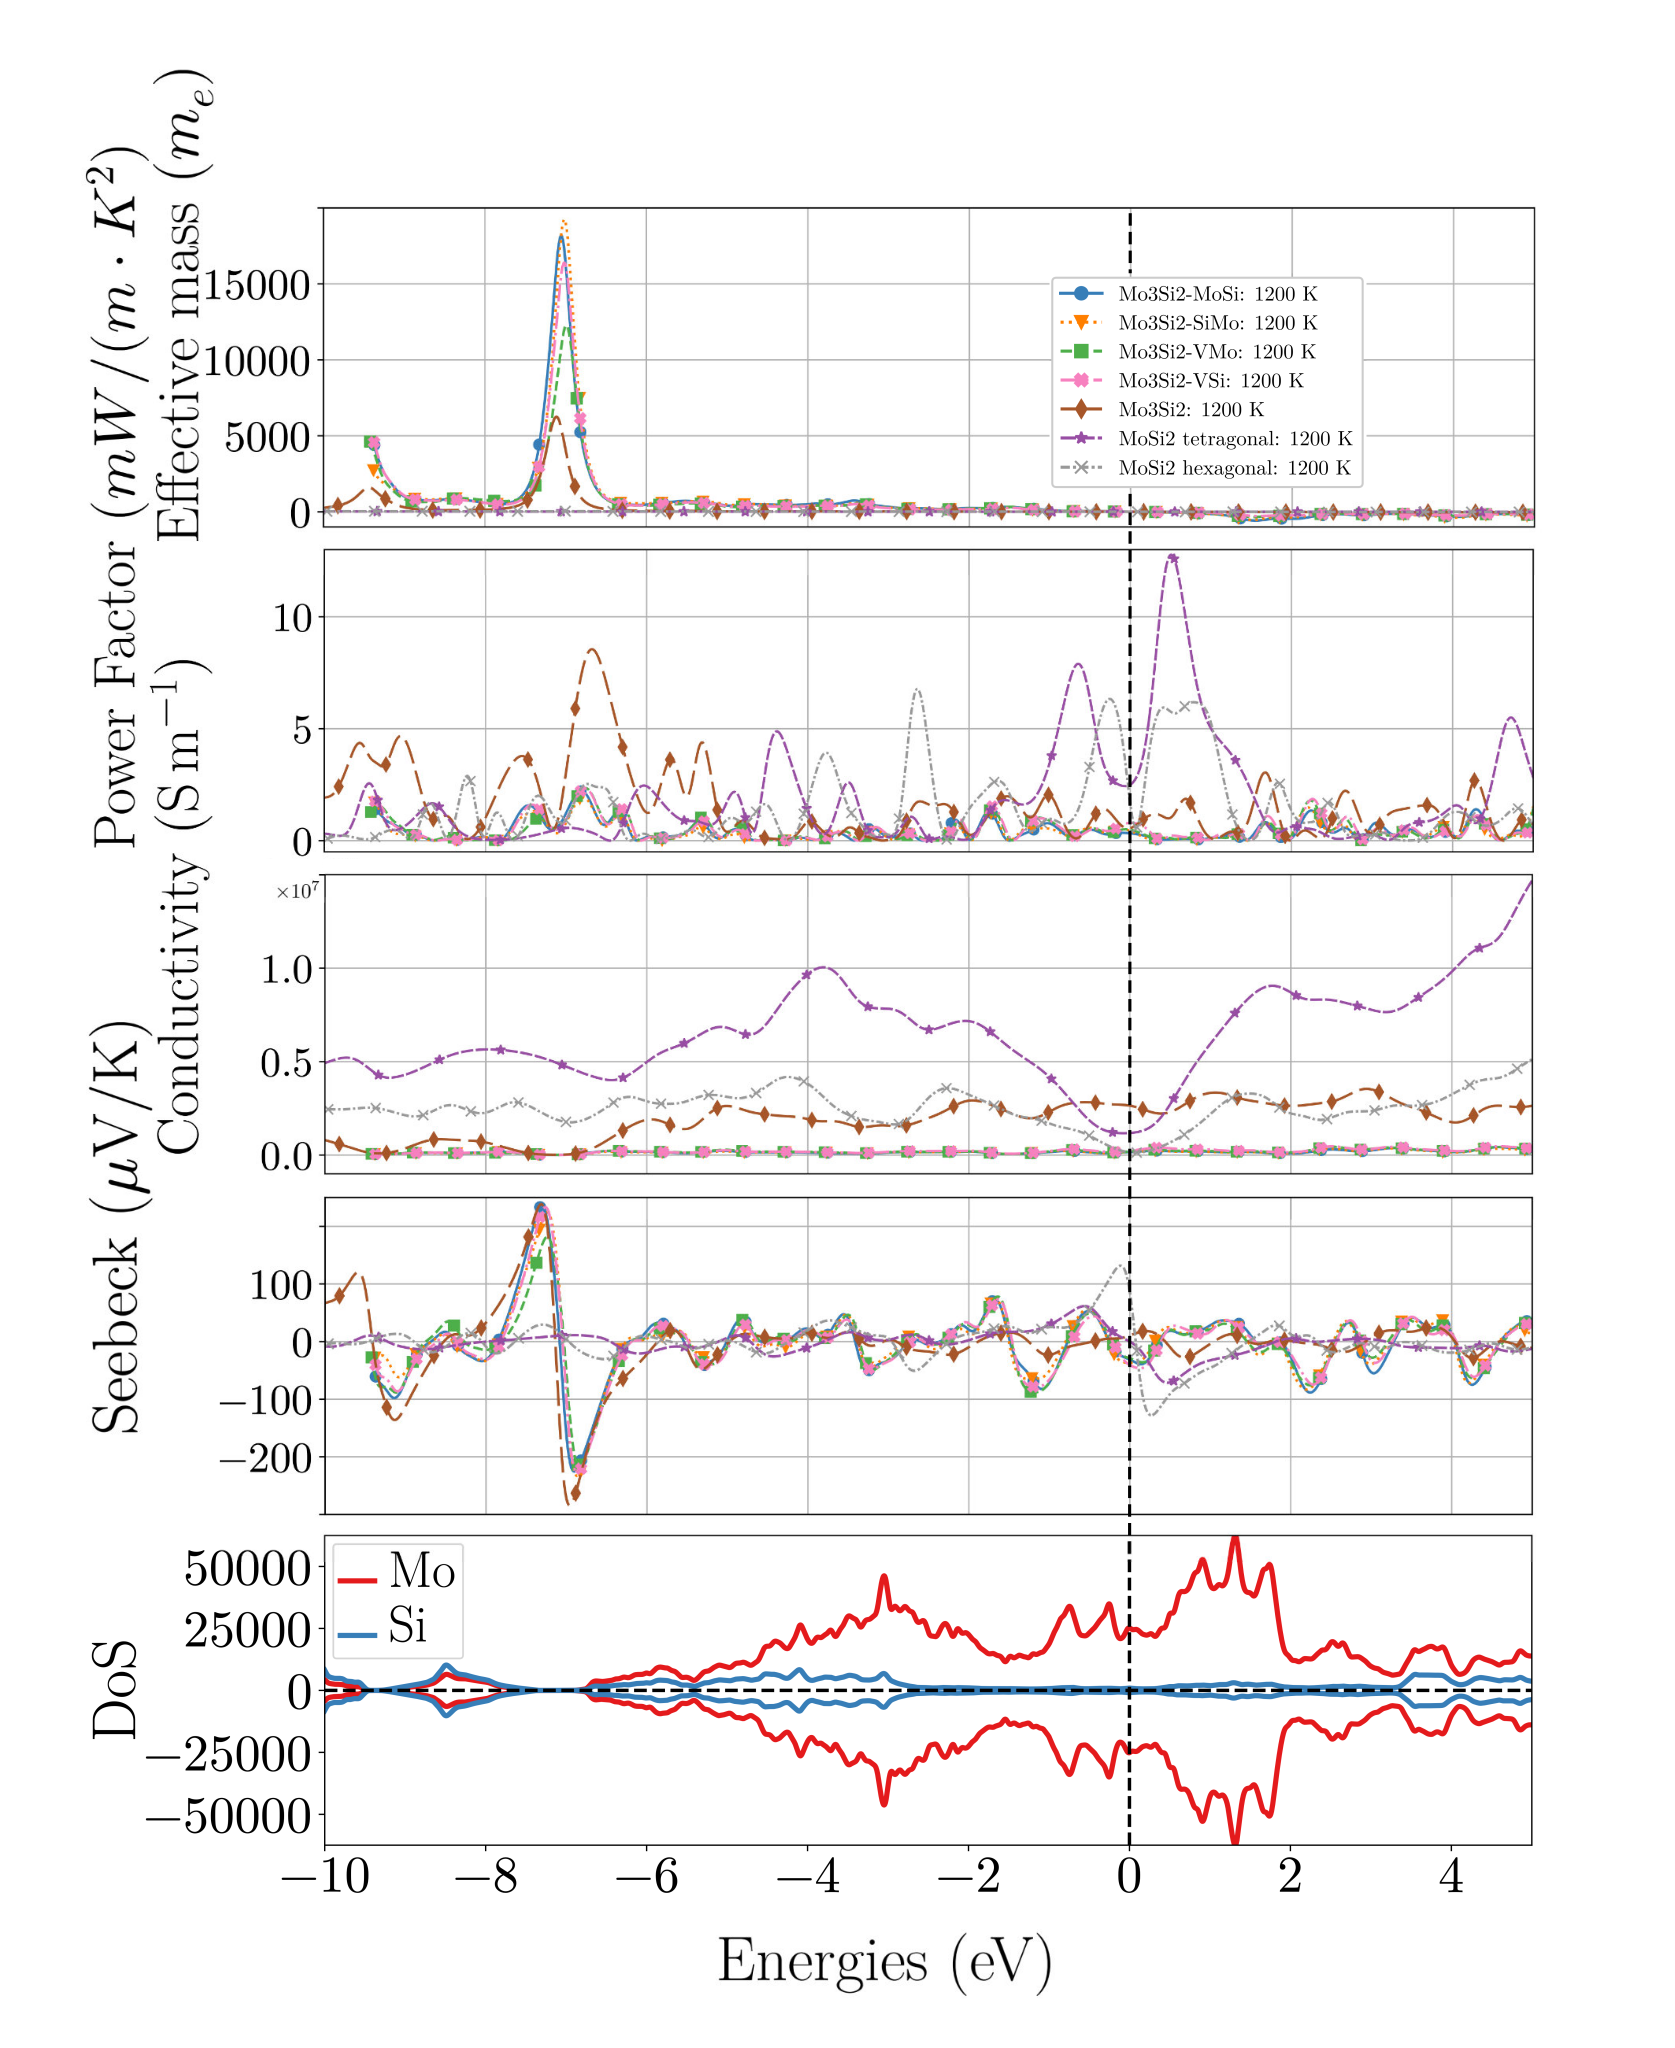
\includegraphics[width=0.8\textwidth]{E-plots}
  \caption{The density of states of silicon and molybdenum is plotted alongside four other quantities on a shared energy axis, where the zero energy is the Fermi energy. The quantities, in order from bottom to top, are the Seebeck coefficient, the conductivity, the power factor and the effective mass. All four quantities each regard the pristine $\text{Mo}\text{Si}_2$ and $\text{Mo}_3\text{Si}_2$ structures, and the four $\text{Mo}_3\text{Si}_2$ defect-containing structures of the latter. The density of states plot is that of pristine $\text{Mo}_3\text{Si}_2$. The DOS of $\text{Mo}\text{Si}_2$ is two orders of magnitude larger in value, and omitted for that reason.}
\label{fig:e-plots}
\end{figure}

\clearpage
\subsection{Density of Electronic States}

\begin{multicols}{2}

\noindent The density of electronic states (DOS) is a measure of the available energy states any given fermionic charge carrier can occupy.
A gap in the DOS corresponds to a gap in the band structure, also referred to as a band gap.
Semi-conductors are identified by the presence of a narrow band gap near the Fermi energy in their DOS; metals have no such gap.

The pristine $\text{Mo}_3\text{Si}_2$ compound has a non-negligible amount of available electronic states at the Fermi energy; this lack of band gap predicts metal-like behaviour (\autoref{fig:e-plots}).
In contrast to this, both $\text{MoSi}_2$ phases have a clearly visible band gap at the Fermi level (\autoref{fig:DOS-mosi2}), indicating that they are semi-conductors.

The density of states corresponding to molybdenum is greater than that corresponding to silicon in all examined compounds, but especially so in the pristine $\text{Mo}_3\text{Si}_2$ structure (\autoref{fig:e-plots}).
In the most extreme case the ratio $\text{DOS}_\text{Mo}/\text{DOS}_\text{Si}$ is approximately 2 for pristine $\text{MoSi}_2$, but the pristine $\text{Mo}_3\text{Si}_2$ structure exhibits a ratio five times as large.
Because there are more available energy states in the Mo sublattice, the mobility of the charge carriers increases on that sublattice.
This positively affects the power factor as it is proportional to the conductivity; therefore, the Mo sublattice is likely the main contributor to the power factor of the $\text{Mo}_3\text{Si}_2$ compounds. 

\end{multicols}

\begin{figure}
\centering
\begin{subfigure}{.5\textwidth}
  \centering
\includegraphics[width=\linewidth]{img/partial_dos_MoSi2_tetragonal.pdf}
  \caption{}
\label{fig:DOS-mosi2-hexagonal}
\end{subfigure}%
\begin{subfigure}{.46\textwidth}
  \centering
\includegraphics[width=\linewidth]{img/partial_dos_MoSi2_hexagonal.pdf}
  \caption{}
\label{fig:DOS-mosi2-tetragonal}
\end{subfigure}
\caption{The partial density of states (DOS) of the pristine tetragonal (a) and hexagonal (b) $\text{Mo}\text{Si}_2$ structures, with the DOS on the y-axis and the electronic energy on the x-axis. The Fermi energy is the zero energy.}
\label{fig:DOS-mosi2}
\end{figure}


% TODO motivate defect formation energy
% - why we plot it
% - discuss

\clearpage
\subsection{Defect Concentration and Formation}

% TODO tetragonal? Pristine? Hexagonal?
\begin{table}[t!]
\caption{The defect formation energies of both MoSi\textsubscript{2} and Mo\textsubscript{3}Si\textsubscript{2} in eV.}
\centering
\begin{tabular}{@{}lllll@{}}
\toprule
      & V\textsubscript{Si}  & V\textsubscript{Mo}  & Mo\textsubscript{Si} & Si\textsubscript{Mo} \\ \midrule
MoSi\textsubscript{2} & 0.71 & 2.83 & 2.91  & 4.80  \\
Mo\textsubscript{3}Si\textsubscript{2} & 1.66 & 0.77 & 2.02  & 1.43 
\end{tabular}
\end{table}

\begin{multicols}{2}

\noindent The defect formation energy is the total energy that is added or released by the introduction of a defect to a given structure. 
A high defect formation energy decreases the equilibrium defect concentration. 
Defect concentrations converge at sufficiently high temperatures (\autoref{eq:defectconcentration}), which follows naturally from Maxwell–Boltzmann statistics.

The intrinsic defect concentrations partly determine the carrier concentrations in undoped systems \cite{carriertemp}. 
These concentrations are directly dependent on the formation energy (\autoref{eq:formationenergy}), which in turn depends on the binding energies of the atoms and the pristine and defective system energy.
% TODO this does not follow from the above
The carrier concentration will ultimately affect both the Seebeck coefficient and the conductivity.

% TODO rewrite!

The silicon vacancies are the most prevalent of the defects in $\text{MoSi}_2$, ranging in concentrations from $10^{-12}$ to $10^{-2}$ mol defects per mol. 
For $\text{Mo}_3\text{Si}_2$ the most frequently occurring defect is the molybdenum vacancy. 
Out of the defects studied, these vacancies may therefore contribute the most to the carrier concentration and the ratio between n- and p-type carriers.
The contrast in defect concentrations between the two compounds is attributed to the difference in material structure, location of the atoms on the lattice, and the defect-induced strain on the lattice.

The defective structures consist of 160 lattice sites, one of which being the point defect itself, resulting in a defect concentration of approximately $10^{-2}$ mol defects per mol. 
At and below the temperature of 2000 K, concentrations similar to those of the simulated samples only occur for the vacancies with the highest equilibrium concentrations (\autoref{fig:defect-form-temp}). 
Therefore, a study on these two vacancy-defected structures would be the most indicative for the  properties of these materials as they are applied in thermoelectric devices.

% REPHRASE - this is copied from a source
% There is an important correlation between the conduction type and the carrier concentration of intrinsic point defects and the negativity $\chi$ and covalent radius $r$ of cations and anions.  This corraletion is referred to by $(\chi ,r)$-mechanism.  The smaller the difference in $\chi$ and $r$ between the cation and the anion the easier it is for antisite defects to form.  On the other hand, increasing the difference will favor the formation of anion vacancies.
% Vacancies can also often be problematic, either resulting in overdoping or by acting as carrier traps that prevent consistent or sufficient doping.

\end{multicols}

\begin{figure}
\centering
\begin{subfigure}{.5\textwidth}
  \centering
  \includegraphics[width=\linewidth]{mosi2defects-zoomed-in}
  \caption{}
  \label{fig:sub1}
\end{subfigure}%
\begin{subfigure}{.5\textwidth}
  \centering
  \includegraphics[width=\linewidth]{mo3si2defects-zoomed-in}
  \caption{}
  \label{fig:sub2}
\end{subfigure}
\caption{The defect concentration as a function of temperature for MoSi\textsubscript{2} (a)  and Mo\textsubscript{3}Si\textsubscript{2} (b). Take due note of the y-axis scale.}
\label{fig:defect-form-temp}
\end{figure}

\clearpage
\pagebreak

\subsection{Transport Properties}

\subsubsection{The Seebeck Coefficient}

% TODO motivate
% - how do the defects effect it?

\begin{multicols}{2}

\noindent The induced voltage in thermoelectric materials is caused by the Seebeck effect.
For a thermoelectric to have high performance, it is necessary to maximize this voltage. 

The Seebeck coefficient is given as a function of temperature to identify the ideal operating temperature for each compound (\autoref{fig:S-Temp}).
For all structures the absolute value of the Seebeck coefficient (the thermopower) increases with temperature up until around 1400 K, after which the values tend towards zero (\autoref{fig:S-Temp}).
The thermopower may be related to the space group of the compounds (\autoref{tab:seebeck}).

The Seebeck coefficient for hexagonal $\text{MoSi}_{2}$ is calculated separately for n- and p-type carriers. 
The reason being that semiconductors with a small band gap can not be approximated as purely n- or p-type at high temperatures; the actual Seebeck coefficient is calculated as an average of both Seebeck coefficients, weighed by their respective conductivities: 
$S_\text{tot}=\left(S_{\mathrm{h}} \sigma_{\mathrm{h}}+S_{\mathrm{e}} \sigma_{\mathrm{e}}\right)/\left(\sigma_{\mathrm{h}}+\sigma_{\mathrm{e}}\right)$ \cite{cdi_proquest_reports_1030752835}. 
Not having taken this into account, the temperature dependence of the power factor is not expected to agree with experimental data.
Nonetheless, a Seebeck coefficient of the same order of magnitude as the largest value we calculated (\autoref{tab:seebeck}) was found experimentally for the hexagonal phase of $\text{MoSi}_{2}$; the experiment determined $S_\text{max}$ for the hexagonal phase to be 89 $\mu\text{V/K}$ at 725 K \cite{YAMADA2011908}.

\end{multicols}

\begin{table}[t!]
  \small
  \centering
  \caption{Largest predicted Seebeck coefficient, evaluated at a carrier concentration of $1.00 \times 10^{21}$ cm$^{-3}$ for each compound, and taken as an absolute value. Most of the values are roughly independent of the defect type. There is a clear correlation between the space group and the thermopower, but the data is insufficient for generalized conclusions.}
\begin{tabular}{@{}lllll@{}}
\toprule
\text {Compound} & \text{space group} & \text{$|S_{\text{max}}|$ ($\mu$V/K)} & \text{$T$ (K)} & \text{Doping} \\
\midrule
\text{Mo}_3\text{Si}_2\text{ prist.} & \text{P4/mbm (number 127)} & 15 & 1800 & \text{n}  \\
\text{Mo}_3\text{Si}_2\text{-MoSi} & \text{Amm2 (number 38)} & 35 & 1200 & \text{n}  \\
\text{Mo}_3\text{Si}_2\text{-SiMo} & \text{Amm2 (number 38)} & 38 & 1200 & \text{n}  \\
\text{Mo}_3\text{Si}_2\text{-VMo} & \text{Amm2 (number 38)} & 30 & 1200 & \text{n}  \\
\text{Mo}_3\text{Si}_2\text{-VSi} & \text{Amm2 (number 38)} & 44 & 1200 & \text{n}  \\
\text{Mo}\text{Si}_2\text{ prist. tetragonal} & \text{I4/mmm (number 139)} & 28 & 1800 & \text{n}  \\
\text{Mo}\text{Si}_2\text{ prist. hexagonal} & \text{P6-222 (number 180)} & 125 & 900 & \text{n}
\end{tabular}
  \label{tab:seebeck}
\end{table}

\begin{figure}
\centering
\begin{subfigure}{.5\textwidth}
  \centering
  \includegraphics[width=\linewidth]{allmats_S_temp_doping_n}
  \caption{}
  \label{fig:sub1}
\end{subfigure}%
\begin{subfigure}{.5\textwidth}
  \centering
  \includegraphics[width=\linewidth]{allmats_S_temp_doping_p}
  \caption{}
  \label{fig:sub2}
\end{subfigure}
\caption{The Seebeck coefficient as a function of temperature at a carrier concentration of $1.00 \times 10^{21}$ cm$^{-3}$ for n-type (a) and p-type (b) doping.}
\label{fig:S-Temp}
\end{figure}

\clearpage
\subsubsection{Electronic Conductivity}

\begin{multicols}{2}

% TODO motivate
% - what is it?
% - why do we plot it?
% - how do the defects effect it?

\noindent The electric conductivity does not strongly depend on temperature, especially so for the defective systems (\autoref{fig:C-Temp}).  
This may be attributed to the absence of phonon interactions in the simulations performed by BoltZTraP2, which dominate conductivity above 100 K \cite{cdi_proquest_reports_1030752835}. 
The total conductivity is the sum of the conductivities caused by both carrier types, $\sigma_{tot} = \sigma_h + \sigma_e$. 
Because the ratio between the densities of the carrier types was not known, the total conductivity could not be determined. 
The defects negatively impact the conductivity for all defective structures; this may be attributed to the large concentration of defects in this material, adding perturbations in the lattice from which electrons scatter. 

The conductivity increases at high carrier concentrations for both phases of $\text{Mo}\text{Si}_{2}$ (\autoref{fig:C-Doping}).
This is expected for semiconducting materials, since the higher carrier concentration populating the conducting band increases the conductivity; and it directly affects the power factor as it is proportional to the conductivity.
This effect seems to be stronger in the tetragonal phase. 

The $\text{Mo}_{3}\text{Si}_{2}$ materials have a roughly constant conductivity with respect to carrier concentration (\autoref{fig:C-Doping}).
The defect-containing $\text{Mo}_{3}\text{Si}_{2}$ structures all have a lower conductivity than the pristine structure (\autoref{fig:C-Doping}).

% [band gap visible from increase in conductivity near 10^21]
% [compare conductivity with formulas from slides]
% [carrier conc. physical at 10^23]

\end{multicols}

\begin{figure}
\centering
\begin{subfigure}{.5\textwidth}
  \centering
  \includegraphics[width=\linewidth]{allmats_C_doping_temp_n}
  \caption{}
  \label{fig:sub1}
\end{subfigure}%
\begin{subfigure}{.5\textwidth}
  \centering
  \includegraphics[width=\linewidth]{allmats_C_doping_temp_p}
  \caption{}
  \label{fig:sub2}
\end{subfigure}
\caption{The conductivity as a function of carrier concentration at a temperature of 1800 K for n-type (a) and p-type (b) doping.}
\label{fig:C-Doping}
\end{figure}

\clearpage
\subsubsection{Effective Mass}

% TODO motivate
% - how do the defects effect it?

\begin{multicols}{2}

\noindent A high induced voltage over a thermoelectric material can only be utilized if energy can be moved, therefore it is of interest to optimize this conductivity for temperature (\autoref{fig:E-Temp}) and for carrier concentration (\autoref{fig:E-doping}).
The effective mass of charge carriers is a measure of their mobility: a higher effective mass implies inertia, and a lower value implies higher conductance. 

Peaks in the effective mass apparently correlate with peaks in the derivative of the Seebeck coefficient; although the latter is not graphed, a peak in the derivative is identified as a steep crossing of the x-axis (\autoref{fig:e-plots}).
% what does this imply? ^

The effective mass of the pristine $\text{Mo}_3\text{Si}_2$ structure is consistently significantly lower than that of the other structures (\autoref{fig:e-plots}); given that a low effective mass is desirable, this suggests that the pristine structure performs better as a thermoelectric than the defective structures \cite{alma9939162912205131}.
A supplementary figure is included in the appendix (\autoref{fig:E-mu}) to compensate for the poor readability of the effective mass in \autoref{fig:e-plots}.

The effective mass of all $\text{Mo}_3\text{Si}_2$ compounds peaks significantly at around 7 eV below the Fermi energy, where the density of electronic states is at a minimum (\autoref{fig:e-plots}). 
The charge carriers lack physical energy states to occupy at that region, which by Fermi's Golden Rule leads to a decrease in charge carrier mobility and as such, a higher effective mass. 
This is also in accordance with the curvature of the band gaps of $\text{Mo}_3\text{Si}_2$ at these energy levels; the effective mass, $m^*=\hbar^2\left(d^2 E(k) / d k^2\right)^{-1}$, is inversely proportional to the electronic band curvature.
This peak does not impact the conductive properties of $\text{Mo}_3\text{Si}_2$ since it is far from the Fermi surface.
% TODO verify with DOS plot of $\text{MoSi}_2$; possible logic error
This is further validated by the lack of peak in the $\text{MoSi}_2$ compounds at the same region, and by the negative effective mass in the densest region for energy states (\autoref{fig:e-plots}).

The effective mass of all compounds and for all defect types grows exponentially with carrier concentration (\autoref{fig:E-doping}).
Most compounds additionally peak in effective mass outside the temperature range of 600 K to 1800 K; with the exception of the hexagonal phase of $\text{MoSi}_2$, p-doped $\text{Mo}_3\text{Si}_2$-$\text{Mo}_{\text{Si}}$ and of p-doped $\text{Mo}_3\text{Si}_2$-$\text{V}_\text{Si}$.
The former peaks at a temperature of 1200 K and the latter two at 900 K.

\end{multicols}

\begin{figure}
\centering
\begin{subfigure}{.5\textwidth}
  \centering
  \includegraphics[width=\linewidth]{allmats_E_doping_temp_n}
  \caption{}
  \label{fig:sub1}
\end{subfigure}%
\begin{subfigure}{.5\textwidth}
  \centering
  \includegraphics[width=\linewidth]{allmats_E_doping_temp_p}
  \caption{}
  \label{fig:sub2}
\end{subfigure}
\caption{The effective mass as a function of carrier concentration at a temperature of 1800 K for n-type (a) and p-type (b) doping.}
\label{fig:E-doping}
\end{figure}

\clearpage
\subsubsection{Power Factor}

% TODO motivate
% - how do the defects effect it?

\begin{multicols}{2}

\noindent A high power factor implies a high figure of merit (\autoref{eq:zt}); the latter being an adequate criteria for thermoelectric materials \cite{alma9939162912205131}.
As we neglect the phonon thermal conductivity, which is non-negligible for high temperatures, we optimize the power factor instead of $zT$ \cite{ZhuTiejun2016NIiI}.
Knowing the temperature at which the power factor is at a maximum is of interest to the engineers (\autoref{fig:Po-T}); furthermore $zT$ implicitly depends on the carrier concentration, and as such it is also relevant to determine its effect on the power factor (\autoref{fig:Po-doping}).

The power factor is possibly correlated with the structure's space group (\autoref{tab:powerfactor}), which is not surprising given the dependence on the Seebeck coefficient; it also appears to depend on temperature, increasing as the temperature rises (\autoref{fig:Po-T}).
The power factor of all the defect-containing $\text{Mo}_3\text{Si}_2$ structures and the hexagonal phase of pristine $\text{MoSi}_2$ peaks in the temperature range of 600 K to 1800 K, but the power factor of the tetragonal phase, and that of pristine $\text{Mo}_3\text{Si}_2$ peaks at a temperature greater than 1800 K (\autoref{fig:Po-T}).

The tetragonal phase of $\text{Mo}\text{Si}_{2}$ seems to have the most favourable power factor for temperatures over 1200 K for n-doped compounds at the chosen carrier concentration (\autoref{fig:Po-T}); the p-doped hexagonal phase has the highest power factor. 
% CONCLUSION: this might mean that an optimal zT is achieved at greater temperatures still. 

These results are unlikely to adequately reflect experimental data for two reasons. 
First, the constant relaxation time approximation was used, which does not take the temperature dependence of the conductivity and of the Seebeck coefficient into account.
And second, the Seebeck coefficient and the conductivity were calculated for both carrier types separately as the carrier concentrations were not known, and both were used for calculating separate n- and p-type dominated power factors.
This implicitly assumes that the material is dominated by either n- or p-type carriers; an assumption that does not hold at high temperatures and in the presence of small band gaps. 
The bipolar effect and the effect of vacancies on the carrier concentrations can not be left out \cite{cdi_proquest_reports_1030752835}.


% The competing structure, hexagonal $\text{MoSi}_{2}$, can be tuned to have a Seebeck coefficient that is almost twice as high as that of the tetragonal $\text{Mo}\text{Si}_{2}$ structure at a carrier concentration of around $10^{21}$ $\text{cm}^{-3}$. Additionally in this range, the conductivity in these materials is much higher. The increase of both parameters would positively affect the power factors for these materials. It is evident from the Figures \ref{fig:S-Doping} and \ref{fig:C-Doping} that these two materials would serve better as n-type semiconductors than p-type semiconductors.

\end{multicols}

\begin{table}[t!]
  \small
  \centering
  \caption{Largest predicted power factor, evaluated at a carrier concentration of $1.00 \times 10^{21}$ cm$^{-3}$ for each compound. The power factor shows a correlation with the structure's space group. Although that could be explained away by the conductivity dependence, the dependence on the thermopower which also exhibits this correlation serves to illustrate the semantic validity of this relation. Some values are roughly independent of the defect type.}
\begin{tabular}{@{}lllll@{}}
\toprule
\text {Compound} & \text{Space group} & \text{Max Power Factor ($m$W/m\cdot $\text{K}^2$)} & \text{$T$ (K)} & \text{Doping} \\
\midrule
\text{Mo}_3\text{Si}_2\text{ prist.} & \text{P4/mbm (number 127)} & 1.5 & 1800 & \text{n or p}  \\
\text{Mo}_3\text{Si}_2\text{-MoSi} & \text{Amm2 (number 38)} & 0.4 & 1200 & \text{n or p}  \\
\text{Mo}_3\text{Si}_2\text{-SiMo} & \text{Amm2 (number 38)} & 0.5 & 1200 & \text{p}  \\
\text{Mo}_3\text{Si}_2\text{-VMo} & \text{Amm2 (number 38)} & 0.5 & 1200 & \text{p}  \\
\, text{Mo}_3\text{Si}_2\text{-VSi} & \text{Amm2 (number 38)} & 0.8 & 1200 & \text{n or p}  \\
\text{Mo}\text{Si}_2\text{ prist. tetragonal} & \text{I4/mmm (number 139)} & 7.7 & 1800 & \text{n}  \\
\text{Mo}\text{Si}_2\text{ prist. hexagonal} & \text{P6-222 (number 180)} & 6.2 & 1500 & \text{p}
\end{tabular}
  \label{tab:powerfactor}
\end{table}

\begin{figure}
\centering
\begin{subfigure}{.5\textwidth}
  \centering
  \includegraphics[width=\linewidth]{allmats_Po_temp_doping_n}
  \caption{}
  \label{fig:sub1}
\end{subfigure}%
\begin{subfigure}{.5\textwidth}
  \centering
  \includegraphics[width=\linewidth]{allmats_Po_temp_doping_p}
  \caption{}
  \label{fig:sub2}
\end{subfigure}
\caption{The power factor as a function of temperature at a carrier concentration of $1.00 \times 10^{21}$ cm$^{-3}$ for n-type (a) and p-type (b) doping.}
\label{fig:Po-T}
\end{figure}

\begin{figure}
\centering
\begin{subfigure}{.5\textwidth}
  \centering
  \includegraphics[width=\linewidth]{allmats_Po_doping_temp_n}
  \caption{}
  \label{fig:sub1}
\end{subfigure}%
\begin{subfigure}{.5\textwidth}
  \centering
  \includegraphics[width=\linewidth]{allmats_Po_doping_temp_p}
  \caption{}
  \label{fig:sub2}
\end{subfigure}
\caption{The power factor as a function of carrier concentration at a temperature of 1800 K for n-type (a) and p-type (b) doping.}
\label{fig:Po-doping}
\end{figure}

\clearpage
\section{Conclusion}

\begin{multicols}{2}

\noindent In this paper we studied the power factor of two molybdenum silicides at high temperatures: $\text{Mo}_3\text{Si}_2$ and $\text{MoSi}_2$. 
We performed computational analysis on previously acquired band energy data obtained through Density Functional Theory. 
The transport properties were examined as a function of carrier density, temperature, and chemical potential; and the data was analyzed to find the most favourable thermoelectric material structure, regarding both p- and n-type materials at high temperatures. 

The stability of each of the point defects was determined by the calculated equilibrium defect concentration. 
We found that the equilibrium concentration of defects with the lowest formation energies matched that of the simulated structures at high temperatures. 
Both the concentrations of the defected samples, and equilibrium defect concentrations for the silicon vacancy in $\text{MoSi}_2$ and the molybdenum vacancy in $\text{Mo}_3\text{Si}_2$ were in the order of $10^{-2}$ mol defects per mol near 1800 K (\autoref{fig:defect-form-temp}).

In both n- and p-type materials, the power factor of the $\text{Mo}_3\text{Si}_2$ structures was significantly lower than that of the tetragonal phase of $\text{MoSi}_{2}$ at all but the very highest carrier concentrations. 
At a carrier concentration of $1.00 \times 10^{21}$ cm$^{-3}$, $\text{MoSi}_2$ had the highest power factor of all studied structures.
The power factor was found to be heavily dependant on temperature (\autoref{fig:Po-T}), which is particularly remarkable given that phonon scattering was not accounted for. 
This temperature dependence is mainly attributed to the temperature dependence of the Seebeck coefficient. 
In choosing the material for a thermoelectric device, the choice should therefore be informed by the operating temperature of said device.

The introduction of molybdenum or silicon vacancies or antisites negatively affected the power factor and most other transport properties of $\text{Mo}_3\text{Si}_2$.
The thermopower remained approximately the same, but the Seebeck coefficient was observed to change sign (\autoref{tab:seebeck}, \autoref{fig:S-Temp}).

% - include relevance of findings in this this paper to future studies.
% - Effect of differing MoxSiy pristine phases on electronic structure and transport properties 

% \autoref{fig:Po-T} additionally shows that at low temperatures, point defects may increase the power factor of the thermoelectric material. $Based on the power factor we found for $\text{Mo}_3\text{Si}_2$ was low compared to that of $\text{MoSi}_2$ for high temperatures. The defective structures of $\text{Mo}_3\text{Si}_2$ where had an even lower power factor in the same temperature ranges. In conclusion it seems that based on the power factors we calculated that $\text{Mo}_3\text{Si}_2$ is not suitable as a thermoelectric Will clean up when back in 3 hours 16:55$

\end{multicols}

\smallskip

\section{Future Studies}

\begin{multicols}{2}

\noindent There are many ways this study could be improved upon. 
The effect of the separate defects could be studied at lower concentrations that better reflect the equilibrium defect concentrations at lower temperatures, specifically T < 1200.
This requires a larger sample size, because the minimum possible defect concentration decreases with increasing sample size; this would significantly increase the computational power required to perform DFT simulations. 
Additionally, since $\text{Mo}_{3}\text{Si}_{2}$ is metallic, the point defects did not alter the relation between the Seebeck coefficient and the carrier concentration significantly, aside from changing sign. 
Further research is needed to study the effect of point defects on molybdenum silicides as semi-conductors or semi-metals. 

Another way to improve on this study is to include the phonon contribution to the Seebeck coefficient and transport properties, which could improve the agreement between our model and experimental data and allow for the study of the figure of merit. 
Phonon contribution to transport properties can be accounted for by implementing a momentum relaxation time approximation \cite{Ganose2021}.

In this study we took the carrier concentrations and temperature of the materials as free parameters; we optimised the Seebeck coefficient by choosing an arbitrary carrier concentration and varying the temperature. 
However, the carrier concentration is dependent on both temperature and defect concentration \cite{carriertemp}. 
In future studies, it would be useful to explore the carrier concentration as a function of temperature and use this relation to optimize the Seebeck coefficient and power factor.

Quantifying defect concentrations is necessary in studies where the effect of defect concentrations on the transport properties are experimentally determined.
The High Harmonic Generation research group at the Advanced Research Center for Nanolithography (ARCNL) has demonstrated a method that could be used for characterising the defects in the volume of a thermoelectric material. 
This group used coherent extreme-ultraviolet pulses from high-harmonic generation to produce a spectrogram. Different point defects are expected to manifest as identifying visual signatures. 
This technique is best suited for materials with a band-gap.  \cite{RoscamAbbingSylvianneD.C2022ESaI}. 

The results in this study are based on DFT calculations; the agreement between this study and experimental data depends in part on accuracy of the DOS obtained from the DFT model. Therefore, determining this accuracy experimentally could be useful.
The Materials & Surface Science for EUVL group at ARCNL utilizes X-ray Photoelectron Spectroscopy (XPS) to access density of states information of CuZr thin films, a technique also applicable to the thermoelectrics discussed in this paper \cite{TrogliaAlessandro2022Tmpv}.
During XPS, a sample is subjected to low-energy X-rays (of the order of 1 keV), after which the emitted photoelectrons are analyzed for their kinetic energy with high precision.
It is also possible to monitor the chemical state of the sample with this technique, but most notable is the high resolution of the resulting DOS data \cite{FadleyC.S.1970Edos}. 

\end{multicols}

\smallskip

\section{Author Contribution Statement}

\begin{multicols}{2}

\noindent All authors contributed to advancing the methodology of this paper. 
Marshall was in charge of processing and visualizing DFT data. 
Jaspers assisted in writing the initial draft of the introduction.
Broerse and Marshall were the main authors of this paper.

\end{multicols}

\medskip


\printbibliography


\clearpage

\pagebreak

\appendix

\section{Appendix A - Supplementary Material Structure Information}

\setcounter{figure}{0}
\renewcommand{\thefigure}{\thesection.\arabic{figure}}% defaul \ref and \listoffigures

\begin{figure*}[b!]
\label{fig:mo3si2-defects-a}
\centering
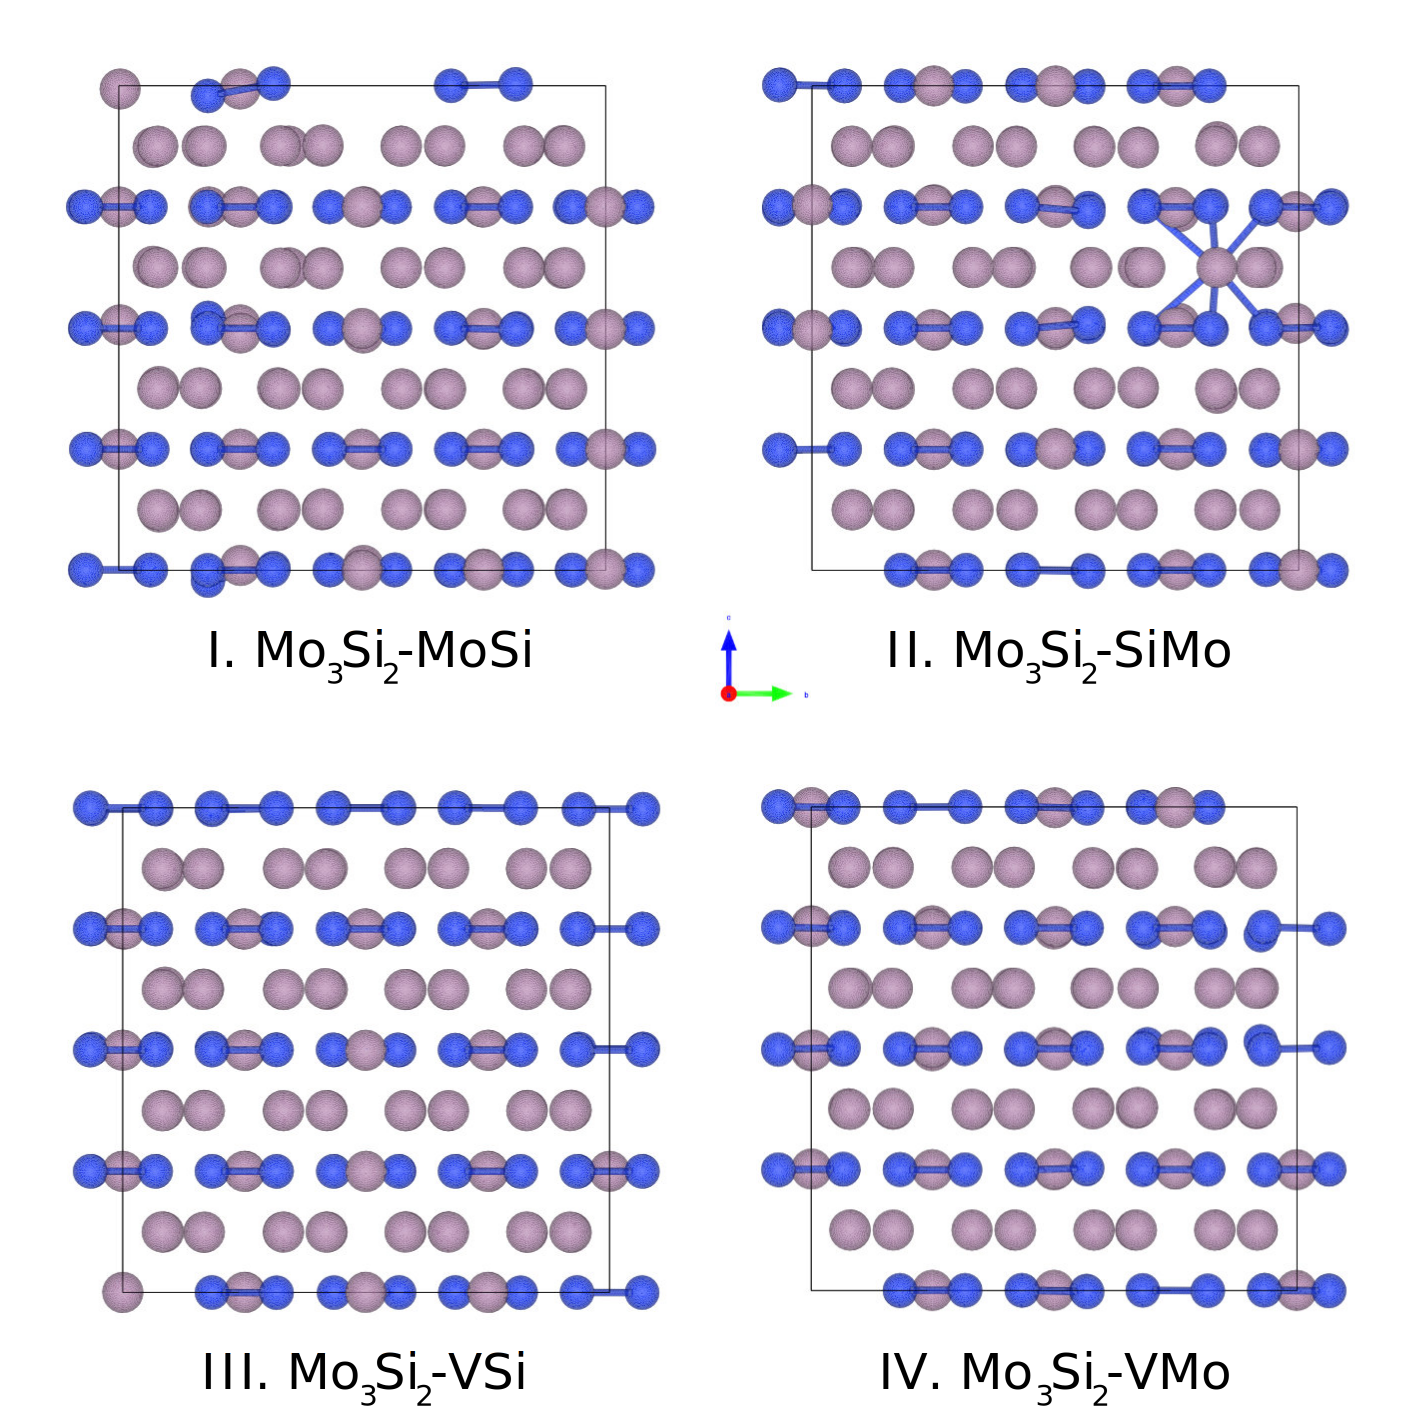
\includegraphics[width=0.6\textwidth]{img/Mo3Si2-defects-a}
\caption{The four defect variants of $\text{Mo}_3\text{Si}_2$ we investigated, all plotted with the $a$ axis facing the camera and the $c$ axis pointing upwards. On the top left corner, the $\text{Mo}_{\text{Si}}$ defect (space group Amm2 number 38), which gives rise to a tilted substructure with respect to the pristine lattice, to be seen on the top-most edge. On the top right corner, the $\text{Si}_{\text{Mo}}$ defect (space group Amm2 number 38), with more strongly bonded atoms than the pristine. On the bottom left corner, the silicon vacancy defect (space group Amm2 number 38); and on the bottom right, the molybdenum vacancy defect (space group Amm2 number 38).}
\end{figure*}

\begin{figure*}[b!]
\label{fig:mo3si2-defects-c}
\centering
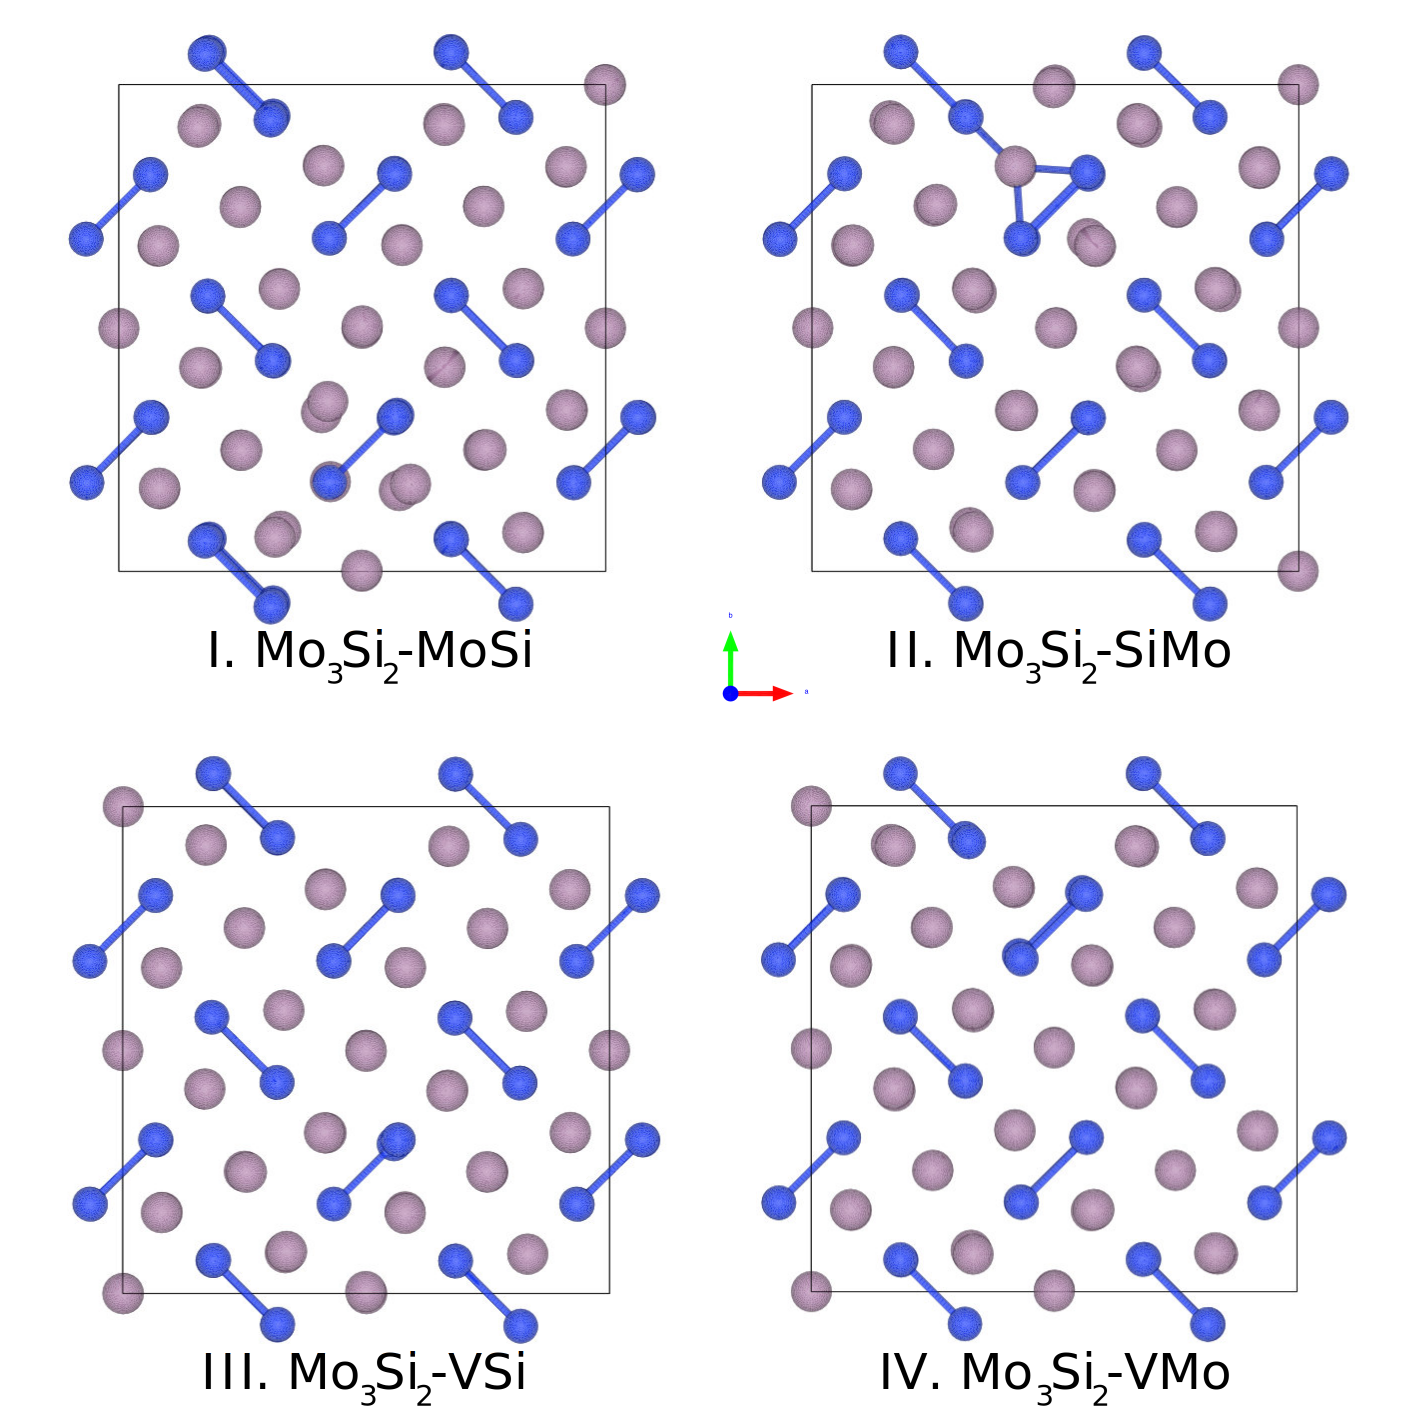
\includegraphics[width=0.6\textwidth]{img/Mo3Si2-defects-c}
\caption{The four defect variants of $\text{Mo}_3\text{Si}_2$ we investigated, all plotted with the $c$ axis facing the camera and the $b$ axis pointing upwards. On the top left corner, the $\text{Mo}_{\text{Si}}$ defect (space group Amm2 number 38). On the top right corner, the $\text{Si}_{\text{Mo}}$ defect (space group Amm2 number 38), with more strongly bonded atoms than the pristine. On the bottom left corner, the silicon vacancy defect (space group Amm2 number 38); and on the bottom right, the molybdenum vacancy defect (space group Amm2 number 38).}
\end{figure*}

\cleardoublepage
\pagebreak
\section{Appendix B - Auxiliary Figures}

\setcounter{figure}{0}
\renewcommand{\thefigure}{\thesection.\arabic{figure}}% defaul \ref and \listoffigures

\subsection{Effective Mass}
\label{appendix:effective-mass}

\begin{figure*}[b!]
\centering
\begin{subfigure}{.5\textwidth}
  \centering
  \includegraphics[width=\linewidth]{allmats_E_temp_doping_n}
  \caption{}
  \label{fig:sub1}
\end{subfigure}%
\begin{subfigure}{.5\textwidth}
  \centering
  \includegraphics[width=\linewidth]{allmats_E_temp_doping_p}
  \caption{}
  \label{fig:sub2}
\end{subfigure}
\caption{The effective mass as a function of temperature at a carrier concentration of $1.00 \times 10^{21}$ cm$^{-3}$ for n-type (a) and p-type (b) carriers.}
\label{fig:E-Temp}
\end{figure*}

\begin{figure*}[b!]
\centering
  \includegraphics[width=\textwidth]{allmats_E_mu_temp_n}
\caption{The effective mass as a function of chemical potential at a temperature of 1800 K.}
\label{fig:E-mu}
\end{figure*}


\pagebreak
\clearpage
\subsection{Conductivity}

\begin{figure*}[b!]
\centering
\begin{subfigure}{.5\textwidth}
  \centering
  \includegraphics[width=\linewidth]{allmats_C_temp_doping_n}
  \caption{}
  \label{fig:sub1}
\end{subfigure}%
\begin{subfigure}{.5\textwidth}
  \centering
  \includegraphics[width=\linewidth]{allmats_C_temp_doping_p}
  \caption{}
  \label{fig:sub2}
\end{subfigure}
\caption{The conductivity as a function of temperature at a carrier concentration of $1.00 \times 10^{21}$ cm$^{-3}$ for n-type (a) and p-type (b) carriers.}
\label{fig:C-Temp}
\end{figure*}

\begin{figure*}[b!]
\centering
  \includegraphics[width=\linewidth]{allmats_C_mu_temp_p}
\caption{The conductivity as a function of chemical potential at a temperature of 1800 K.}
\label{fig:C-mu}
\end{figure*}


\pagebreak
\clearpage
\subsection{Power Factor}

\begin{figure*}[b!]
\centering
\includegraphics[width=\linewidth]{allmats_Po_mu_temp_p}
\caption{The power factor as a function of chemical potential at a temperature of 1800 K.}
\label{fig:Po-mu}
\end{figure*}


\pagebreak
\clearpage
\subsection{The Seebeck Coefficient}

\begin{figure*}[b!]
\centering
\begin{subfigure}{.5\textwidth}
  \centering
  \includegraphics[width=\linewidth]{allmats_S_doping_temp_n}
  \caption{}
  \label{fig:sub1}
\end{subfigure}%
\begin{subfigure}{.5\textwidth}
  \centering
  \includegraphics[width=\linewidth]{allmats_S_doping_temp_p}
  \caption{}
  \label{fig:sub2}
\end{subfigure}
\caption{The Seebeck coefficient as a function of carrier concentration at a carrier concentration of $1.00 \times 10^{21}$ cm$^{-3}$ for n-type (a) and p-type (b) carriers.}
\label{fig:S-Doping}
\end{figure*}

\begin{figure*}[b!]
\centering
\includegraphics[width=\linewidth]{allmats_S_mu_temp_p}
\caption{The Seebeck coefficient as a function of chemical potential at a temperature of 1800 K.}
\label{fig:S-mu}
\end{figure*}

\pagebreak
\clearpage
\subsection{Carrier Concentration}

\begin{figure*}[b!]
\centering
  \includegraphics[width=0.6\textwidth]{mo3si2defects}
  \caption{The defect concentration as a function of temperature for Mo\textsubscript{3}Si\textsubscript{2}, zoomed out onto a broader defect concentration range.}
  \label{fig:carrier-concentration-mo3si2}
\end{figure*}

\begin{figure*}[b!]
\centering
  \includegraphics[width=0.6\textwidth]{mosi2defects}
  \caption{The defect concentration as a function of temperature for MoSi\textsubscript{2}, zoomed out onto a broader defect concentration range.}
  \label{fig:carrier-concentration-mosi2}
\end{figure*}

\cleardoublepage
\pagebreak
\section{Appendix C - Full Band Structure Plots}

\setcounter{figure}{0}
\renewcommand{\thefigure}{\thesection.\arabic{figure}}% defaul \ref and \listoffigures

\begin{figure*}[b!]
\label{fig:bs_Mo3Si2_full}
\centering
\includegraphics[width=\textwidth]{bs_Mo3Si2_full}
\caption{The band structure of the pristine Mo\textsubscript{3}Si\textsubscript{2} structure across high symmetry points, plotted through the full path provided by SeeK-Path.}
\end{figure*}

\begin{figure*}[b!]
\label{fig:bs_MoSi2_hexagonal_full}
\centering
\includegraphics[width=\textwidth]{bs_MoSi2_hexagonal_full}
\caption{The band structure of the hexagonal phase of pristine MoSi\textsubscript{2} across high symmetry points, plotted through the full path provided by SeeK-Path.}
\end{figure*}

\begin{figure*}[b!]
\label{fig:bs_MoSi2_tetragonal_full}
\centering
\includegraphics[width=\textwidth]{bs_MoSi2_tetragonal_full}
\caption{The band structure of the tetragonal phase of pristine MoSi\textsubscript{2} across high symmetry points, plotted through the full path provided by SeeK-Path.}
\end{figure*}

\end{document}

% TODO:
% - write abstract!! do this at last (present, not done)
% - link findings to existing studies: compare to power factors of existing materials
% - figures in correct places, do this at last
% - correct typesetting, do this at last
% - compare binding energy to bond lengths
% - bond angles?
% - verify no faults in bibliography
% - check that methodology links well to what is done in results

% RESULTS TO DISCUSS:
% - Defect formation energies (REQUIRED) 
    - relate defect formation energies to (change in) bond lengths
% - Conductivity (REQUIRED) (present, not done)
% - Power factor (REQUIRED) (present, not done)
% - Transport properties as a function of carrier concentration/T/chemical potential/relaxation time (REQUIRED) (present, not done)
   - justify why we chose to plot x vs y (present in most things)
% - Effect of defects on materials properties (REQUIRED) 

%   - tetra vs hexa, we have them in the plots; discuss

% - the angle change in the defect structure

% CONCLUSION TODO:
% - we also studied point defects in one of the materials, conclude our findings:
    adding defects worked against power factor, mainly because it greatly reduced the coductivity of the material. flipped sign of seebeck coefficient, magnitude and relation 
    not significantly altered. 
% - include relevance of findings in this this paper to future studies.
% - Effect of differing MoxSiy pristine phases on electronic structure and transport properties 

(REQUIRED)

% LOW PRIO TODO:
% - verify values of tables, as they are taken by eye from the plots

% POST PROCESSING TODO, in order:
% - verify appendix references are correct and not missing
% - verify citations are where needed
% - verify citations are correctly printed in the bibliography
% - revise logic flow (clarity)
% - replace mo3si and such things with proper typesetting
% - use correct spelling of coefficient and other such words
% - check workflow
% - consider restructuring
% - reread and be critical of conclusion